\section{Approach}
\label{se:approach}

The key to platform independence in our approach is to encode the entire OSR machinery at intermediate representation level, without resorting to machine-level code manipulation.

\subsection{Overview}

\begin{figure}
\begin{center}
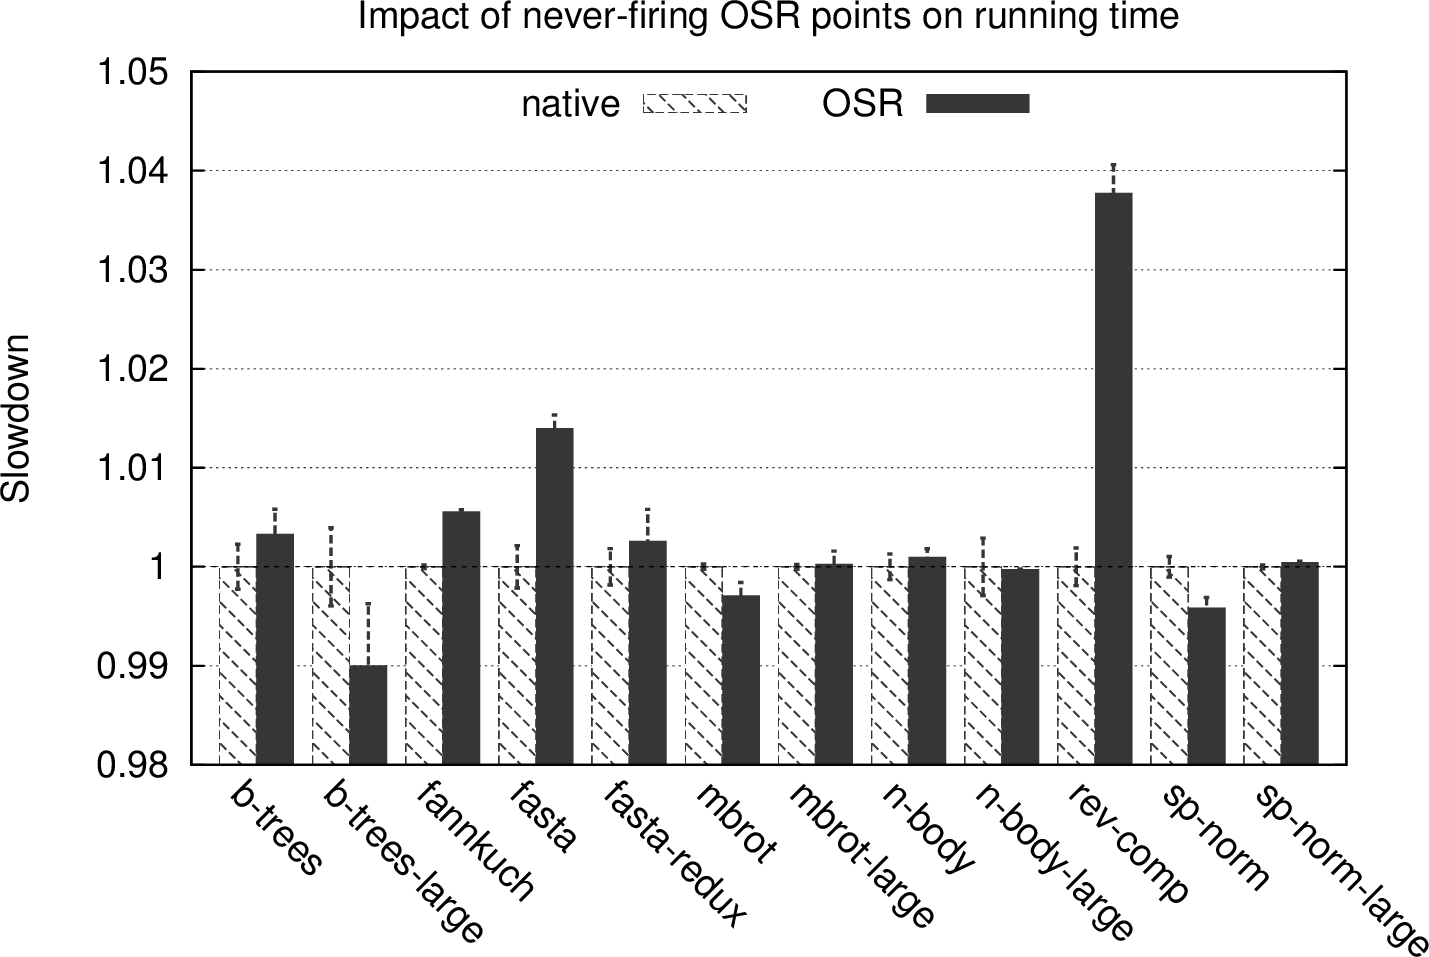
\includegraphics[width=0.7\columnwidth]{figures/code-quality-noBB/code-quality-noBB.png}
\caption{\label{fig:code-quality2} Impact on running time of never-firing OSR points inserted inside hot code portions.}
\end{center}
\end{figure}

%\begin{verbatim}
%int fac(int n) {
%    int i = 2, f = 1;
%    while (i<=n) f *= i++;
%    return f;
%}
%\end{verbatim}
%
%\begin{verbatim}
%int fac(int n) {
%    int i = 2, f = 1;
%    while (i<=n)  {
%        if (osr_cond) return fac_osr(n,i,f); 
%        f *= i++; 
%    } return f;
%}
%\end{verbatim}
%
%\begin{verbatim}
%int fac_osr(int n) {
%    goto L;
%    int i = 2, f = 1;
%    while (i<=n) L: f *= i++;
%    return f;
%}
%\end{verbatim}

\subsection{LLVM API for OSR}

\subsubsection{Finalized OSR Points}

\subsubsection{Open OSR Points}


  
  
  
  
  
  
  
  
  
  
  
  
  
  
  
  
  
  